\begin{frame}
\frametitle{Goals}
\begin{itemize}
\item Our existing common goals
\item The goals for today
\end{itemize}
\end{frame}


\begin{frame}
\frametitle{Goals}
\framesubtitle{Our common goals}
\begin{block}{to implement software efficiently}
\begin{itemize}
\item to arrive at an initial result as quickly as possible
\item over time, to reliably arrive at results as quickly as possible (aka maintenance)
\item a result is valid if the program accurately achieves our objective
% if a result does not achieve our objective, we revise our objective to determine what we have achieved. We not construct a system of apologetics for shortcomings, so as to maintain the illusion of having achieved the goal.
\end{itemize}
\end{block}
\end{frame}


\begin{frame}
\frametitle{Goals}
\framesubtitle{Our common goals}
\begin{block}{impertinent goals}
\begin{itemize}
\item financial gain "but django makes me \$\$\$!"
\item motivate personal avidities
\end{itemize}
\end{block}
\end{frame}


\begin{frame}
\frametitle{Goals}
\framesubtitle{Our goals for today}
\begin{block}{"Why Django Sucks"}
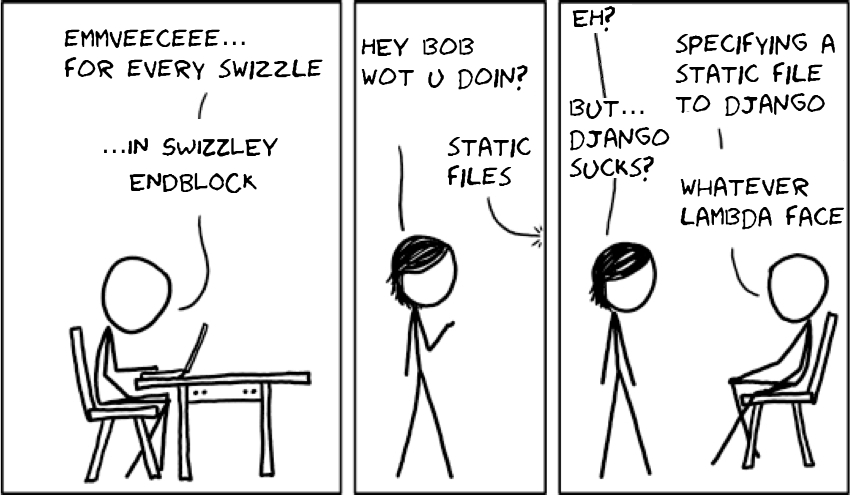
\includegraphics[width=0.7\paperwidth]{image/why-django-sucks.png}
\end{block}
\end{frame}


\begin{frame}
\frametitle{Goals}
\framesubtitle{Our goals for today}
\begin{block}{I could talk all day about why django sucks}
\begin{itemize}
\item<1> and I'd be saying lots and lots of true things
\item<2> but not necessarily helpful things
\end{itemize}
\end{block}
\end{frame}


\begin{frame}
\frametitle{Goals}
\framesubtitle{Our goals for today}
\begin{block}{The goal today}
To equip you with new tools and perspective, with which to explore the question for yourself.
\end{block}
\end{frame}